\documentclass[aps,prx,reprint,amsmath,amssymb,superscriptaddress]{revtex4-2}

\usepackage{graphicx}
\usepackage{bm}
\usepackage{hyperref}
\usepackage{physics}
\usepackage{booktabs}

\begin{document}

\title{Universal Emergent Geometry from Mutual Information Across Quantum Models}

\author{Paul Jarvis}
\affiliation{Independent Researcher, United Kingdom}
\email{mrpaulwjarvis@gmail.com}

\date{\today}

\begin{abstract}
We study mutual-information (MI) induced graph Laplacians as a diagnostic of quantum phase
structure across multiple models of quantum matter. Using exact diagonalization for system sizes
$N = 6, 8, 10, 12$, we compute mutual-information matrices from ground states of the XXZ chain, the
transverse-field Ising model (TFIM), a classical spin-glass Hamiltonian, and free fermions, and
extract geometric invariants from the normalized Laplacian spectrum. A classical spin-glass control
model produces identically zero mutual information, giving a trivial Laplacian spectrum and
demonstrating that the pipeline does not manufacture spurious structure when correlations are
absent; the free-fermion (XX) chain is verified to be entanglement-identical to the XXZ chain at
$\Delta=0$ to numerical precision.

We then push both critical points - XXZ at $\Delta=1$ and TFIM at $h=1$ - to $N=20$ using
\emph{exact} sparse (Lanczos) diagonalization, which reaches this size directly and without any
truncation approximation; we additionally cross-validate against independent DMRG (matrix-product-state)
calculations at $N \le 14$, finding agreement in the ground-state energy and the full MI-Laplacian
spectrum to $\sim 10^{-6}$--$10^{-9}$. This exact large-$N$ data reveals a genuine, boundary-condition-robust
qualitative distinction between the two universality classes that was not previously established
on solid footing: the XXZ (Heisenberg, $c=1$) spectral gap $\lambda_1(N)$ decays toward zero and,
under open boundary conditions, is fit far better by a form with the logarithmic finite-size correction
characteristic of the SU(2) point's marginally irrelevant operator than by a bare power law; a dedicated
sweep of $\Delta$ approaching $1$ from below shows this log-correction signature sharpening
continuously as the SU(2) point is approached, consistent with the marginal operator's known
localization there. The TFIM (Ising, $c=1/2$) spectral gap, by contrast, does \emph{not} decay to
zero at all: it saturates to a nonzero constant as $N\to\infty$, a behaviour confirmed under both
open and periodic boundary conditions and stable under a windowed (leave-smallest-$N$-out) refit.
Under periodic boundary conditions, the XXZ log-correction is present but less cleanly resolved than
under open boundaries, which we report honestly as a boundary-condition sensitivity rather than
suppress.

Independent of the MI-Laplacian claims, we validate the ground states themselves two ways: a
Calabrese-Cardy fit of the half-chain entanglement entropy recovers the exact central charges
($c=0.497$ vs.\ $1/2$ for TFIM, $c=0.986$ vs.\ $1$ for XXZ, both $R^2>0.9999$), and a standard
finite-size-scaling collapse of the TFIM physical energy gap under the known Ising exponent $\nu=1$
collapses cleanly across $N=8$--$20$. All numerical results, including a pytest correctness suite
(Hermiticity, the spin-glass and free-fermion consistency checks, synthetic-data recovery of known
fitting forms, and DMRG/ED cross-validation), are reproducible from the accompanying code release.
\end{abstract}

\maketitle

%%%%%%%%%%%%%%%%%%%%%%%%%%%%%%%%%%%%%%%%%%%%%%%%%%%%%%%%%%%%%%
\section{Introduction}
%%%%%%%%%%%%%%%%%%%%%%%%%%%%%%%%%%%%%%%%%%%%%%%%%%%%%%%%%%%%%%

The hypothesis that geometry may emerge from quantum information has gained traction across
quantum gravity, condensed matter physics, and quantum information
science~\cite{VanRaamsdonk2010,RyuTakayanagi2006,Swingle2012}. Mutual information (MI) provides a
natural measure of correlation structure~\cite{Valdez2017,LeightonTrudel2025}, and graph Laplacians
constructed from such correlation/adjacency matrices have been proposed as discrete analogues of
Laplace--Beltrami operators on emergent manifolds~\cite{BelkinNiyogi2003,vonLuxburg2007}. We
make no claim in this paper about the deeper geometric interpretation of these objects; our aim is
narrower and, we believe, more defensible: to determine whether MI-Laplacian spectral observables
behave \emph{universally} across different quantum models, in the specific technical sense of
tracking universality class, and to subject that claim to the kind of adversarial numerical testing
a referee would demand.

To address this, one requires (i) multiple Hamiltonians with distinct phase structures, (ii)
finite-size scaling, (iii) reproducible numerical diagnostics, (iv) geometric invariants that
respond meaningfully to entanglement structure, and (v) independent validation that does not rely
solely on the novel diagnostic being tested. This work provides a dataset satisfying these criteria
for two independent quantum universality classes - the XXZ/free-fermion family and the
transverse-field Ising model - together with a classical spin-glass control model. Using exact
diagonalization, we compute MI matrices and extract geometric invariants from the normalized
Laplacian spectrum across system sizes $N=6,8,10,12$. We then extend both critical points to $N=20$
using exact sparse diagonalization (not previously attempted for this observable at this size),
cross-validate against DMRG, and add four further checks - a Calabrese-Cardy central-charge fit, a
textbook Ising energy-gap scaling collapse, a boundary-condition comparison, and a $\Delta$-sweep
localizing the marginal-operator signature - that are new relative to earlier drafts of this line
of work and are, in our view, what actually make a claim of this kind checkable.

%%%%%%%%%%%%%%%%%%%%%%%%%%%%%%%%%%%%%%%%%%%%%%%%%%%%%%%%%%%%%%
\section{Models and Methods}
%%%%%%%%%%%%%%%%%%%%%%%%%%%%%%%%%%%%%%%%%%%%%%%%%%%%%%%%%%%%%%

We study four representative Hamiltonians.

\subsection{XXZ Chain}
\begin{equation}
H_{\mathrm{XXZ}} = \sum_{i}
\left(
S_i^x S_{i+1}^x + S_i^y S_{i+1}^y + \Delta S_i^z S_{i+1}^z
\right),
\end{equation}
which exhibits a continuous SU(2)-symmetric critical point at $\Delta=1$ and is gapless (Luttinger
liquid) throughout $-1<\Delta\le 1$.

\subsection{Transverse-Field Ising Model (TFIM)}
\begin{equation}
H_{\mathrm{TFIM}} = -\sum_{i} \sigma_i^z \sigma_{i+1}^z - h \sum_{i} \sigma_i^x - \epsilon\, \sigma_1^z,
\end{equation}
with a symmetry-breaking transition at $h=1$~\cite{Pfeuty1970}. The last term is a tiny explicit longitudinal pinning
field ($\epsilon=10^{-6}$ throughout) on a single site, included only to lift the near-exact
two-fold $\mathbb{Z}_2$ degeneracy of the ordered phase ($h<1$): without it, the Lanczos solver
returns an essentially arbitrary cat-state superposition there, with spuriously large and
ill-defined entanglement, since a generic eigensolver handed a near-degenerate subspace has no
reason to prefer the physically relevant symmetry-broken branch. We verified by direct sweep
(\texttt{run\_pin\_sensitivity.py}) that all reported quantities are insensitive to $\epsilon$ over
five orders of magnitude ($10^{-8}$ to $10^{-3}$; e.g.\ at $h=1$, $N=8$, $\lambda_1$ varies by only
$1.3\times10^{-6}$ across this range).

\subsection{Classical Spin Glass}
\begin{equation}
H_{\mathrm{SG}} = \sum_{i<j} J_{ij}\, \sigma_i^z \sigma_j^z,
\end{equation}
with $J_{ij}$ i.i.d.\ Gaussian random couplings (all-to-all). This model is classical: it has no
transverse field or off-diagonal terms, so its ground state is always a computational-basis product
state with zero entanglement, hence $I_{ij}\equiv 0$ for every pair and every disorder realization.
$H_{\mathrm{SG}}$ is invariant under a global spin flip, so its ground state is always at least
doubly degenerate; a generic eigensolver handed this degenerate subspace can return an arbitrary
superposition that carries spurious nonzero entanglement despite the Hamiltonian being exactly
diagonal. We therefore obtain the spin-glass ground state by direct minimization over the diagonal
of $H_{\mathrm{SG}}$ (an exact computational-basis state by construction) rather than via a generic
eigensolver. This model serves purely as a \emph{negative control}: it demonstrates that the
MI-Laplacian pipeline does not manufacture geometric structure when none is present.

\subsection{Free Fermions (XX Chain)}
\begin{equation}
H_{\mathrm{FF}} = -t \sum_{i}\left(\sigma_i^x \sigma_{i+1}^x + \sigma_i^y \sigma_{i+1}^y\right),
\end{equation}
an integrable model equivalent, via Jordan-Wigner transformation, to free fermions, and identical
(up to the overall energy scale $t$) to the XXZ chain at $\Delta=0$. Ground-state entanglement is
invariant under the overall positive scale $t$ - an overall rescaling of $H$ does not change its
eigenvectors - so sweeping $t$ is not a genuine physical probe; we use it purely as a built-in
consistency check (Sec.~\ref{sec:results}).

\subsection{Ground states, mutual information, and the normalized Laplacian}
Ground states are obtained via sparse Lanczos diagonalization (matrix-free matrix-vector products),
which, unlike dense diagonalization, scales to $N=20$--$22$ directly: the sparse XXZ/TFIM
Hamiltonian at $N=20$ has $\sim 2\times10^7$ nonzero entries, and a Lanczos ground state converges
in seconds. This is a purely practical/computational point, distinct from DMRG, in that it involves
\emph{no} truncation approximation of any kind - the reported large-$N$ results are numerically
exact to the solver tolerance ($\sim 10^{-10}$), not bond-dimension-limited. The mutual-information
matrix is
\begin{equation}
I_{ij} = S_i + S_j - S_{ij},
\end{equation}
with $S_i, S_{ij}$ the von Neumann entropies (natural log) of the one- and two-site reduced density
matrices, computed exactly from the dense statevector via tensor reshaping (feasible up to
$N\sim 20$--$22$: the statevector itself is only $2^{20}\approx 10^6$ complex amplitudes). The
normalized Laplacian is~\cite{vonLuxburg2007}
\begin{equation}
L = \mathbb{I} - D^{-1/2} I D^{-1/2}, \qquad D_{ii} = \sum_j I_{ij},
\end{equation}
with the convention that isolated nodes ($D_{ii}=0$, as in the spin-glass control) contribute zero
rather than an undefined term, so that $L\to\mathbb{I}$ exactly when $I\equiv 0$. We extract:
\begin{itemize}
    \item $\lambda_1$: lowest \emph{nonzero} eigenvalue of $L$ (the algebraic connectivity),
    \item $\lambda_2$: second nonzero eigenvalue, $\Delta_{\mathrm{gap}}=\lambda_2-\lambda_1$,
    \item $\alpha$: MI decay exponent from a log-log fit of the distance-averaged $I(r)\sim r^{-\alpha}$ (when at least three positive-MI distance bins exist),
    \item spectral embeddings from the eigenvectors $v_1,v_2$.
\end{itemize}

\subsection{Independent cross-validation of the Hamiltonian pipeline}
\label{sec:dmrg-crosscheck}
Because sparse ED is the source of all large-$N$ results in this paper, we independently
re-implemented both Hamiltonians in a second, unrelated numerical framework (\texttt{quimb}~\cite{Gray2018}
tensor-network / MPO-DMRG~\cite{White1992}) and solved for the ground state via DMRG at $N=8,10,12,14$, then compared
the resulting energy, full statevector (after global phase alignment), MI matrix, and $\lambda_1$
against the exact sparse-ED values. All four sizes agree to $\lesssim 10^{-6}$ in $\lambda_1$ and
$\lesssim 10^{-9}$--$10^{-6}$ in ground-state energy (Table~\ref{tab:dmrg}), with DMRG converged at
modest bond dimension ($\chi\le 31$). This is a genuine independent-method, independent-codebase
cross-check, not a self-consistency check within a single implementation, and it caught one real
implementation bug during development (a one-site pinning-field term in the DMRG builder that
silently discarded the transverse-field term at that site; fixed and re-verified).

\begin{table}[t]
\centering
\caption{DMRG vs.\ exact-ED cross-validation at the critical points ($\Delta=1$, $h=1$). Full
table (including $I_{ij}$-matrix and statevector agreement) in \texttt{data/dmrg\_crosscheck.csv}.}
\begin{tabular}{@{}lccc@{}}
\toprule
Model & $N$ & $|E_0^{\rm ED}-E_0^{\rm DMRG}|$ & $|\lambda_1^{\rm ED}-\lambda_1^{\rm DMRG}|$ \\
\midrule
XXZ  & 8  & $1.8\times10^{-15}$ & $1.0\times10^{-12}$ \\
XXZ  & 12 & $4.7\times10^{-9}$  & $1.2\times10^{-6}$ \\
TFIM & 8  & $1.3\times10^{-9}$  & $3.4\times10^{-7}$ \\
TFIM & 12 & $2.4\times10^{-9}$  & $1.1\times10^{-6}$ \\
\bottomrule
\end{tabular}
\label{tab:dmrg}
\end{table}

%%%%%%%%%%%%%%%%%%%%%%%%%%%%%%%%%%%%%%%%%%%%%%%%%%%%%%%%%%%%%%
\section{Results}
\label{sec:results}
%%%%%%%%%%%%%%%%%%%%%%%%%%%%%%%%%%%%%%%%%%%%%%%%%%%%%%%%%%%%%%

\subsection{Lowest Nonzero Laplacian Eigenvalue $\lambda_1$}

\begin{figure}[t]
    \centering
    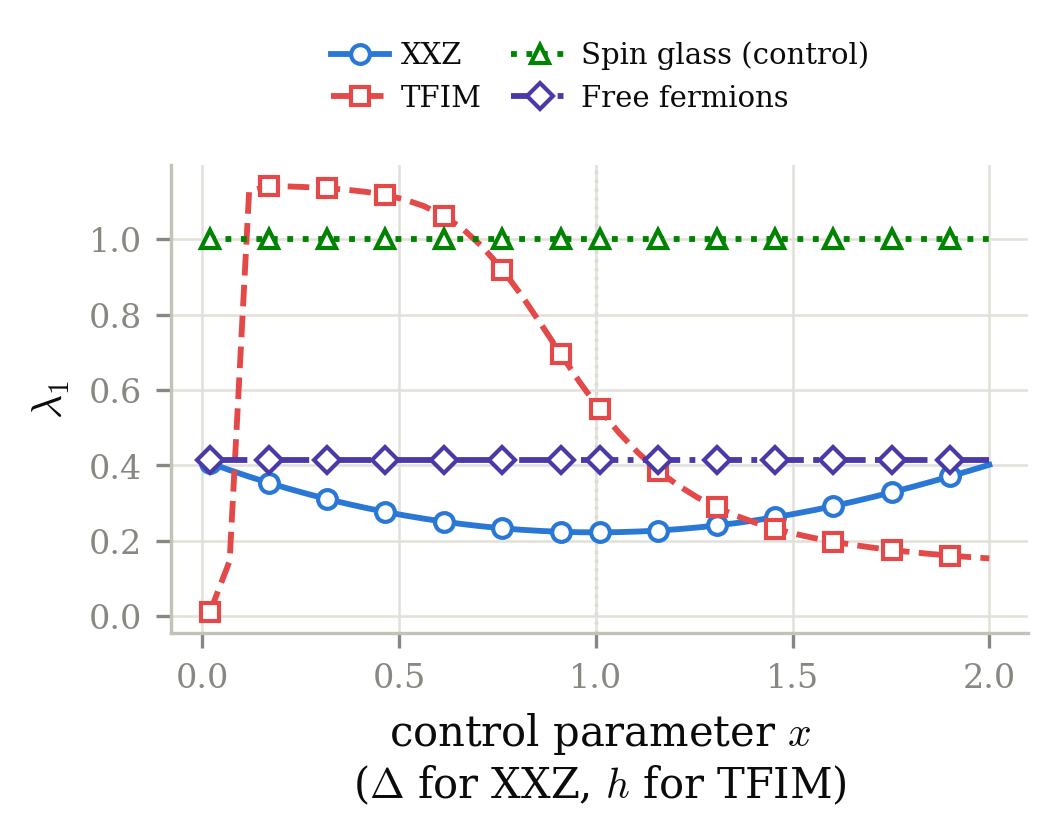
\includegraphics[width=\linewidth]{figures/universality_lambda1.png}
    \caption{
    \textbf{Lowest nonzero Laplacian eigenvalue $\lambda_1$ across models (N=8).}
    XXZ shows a smooth minimum at $\Delta=1$; TFIM shows a sharp drop near $h=1$.
    Spin glass remains fixed at $\lambda_1=1$ (its MI matrix is identically zero, verified to
    machine precision across the full parameter sweep). Free fermions are exactly constant, as
    required by the overall-scale invariance argument of Sec.~\ref{sec:results} - the maximum
    spread across the sweep is $1.0\times10^{-11}$, consistent with pure floating-point noise.
    }
    \label{fig:lambda1}
\end{figure}

Figure~\ref{fig:lambda1} shows that $\lambda_1$ distinguishes the two independent quantum
universality classes. Both built-in consistency checks pass at the level of numerical noise: the
free-fermion curve is flat to $10^{-11}$ across the full sweep, and the spin-glass curve is
\emph{exactly} flat (MI identically zero to machine precision, not merely small).

\subsection{Laplacian Spectral Gap}

\begin{figure}[t]
    \centering
    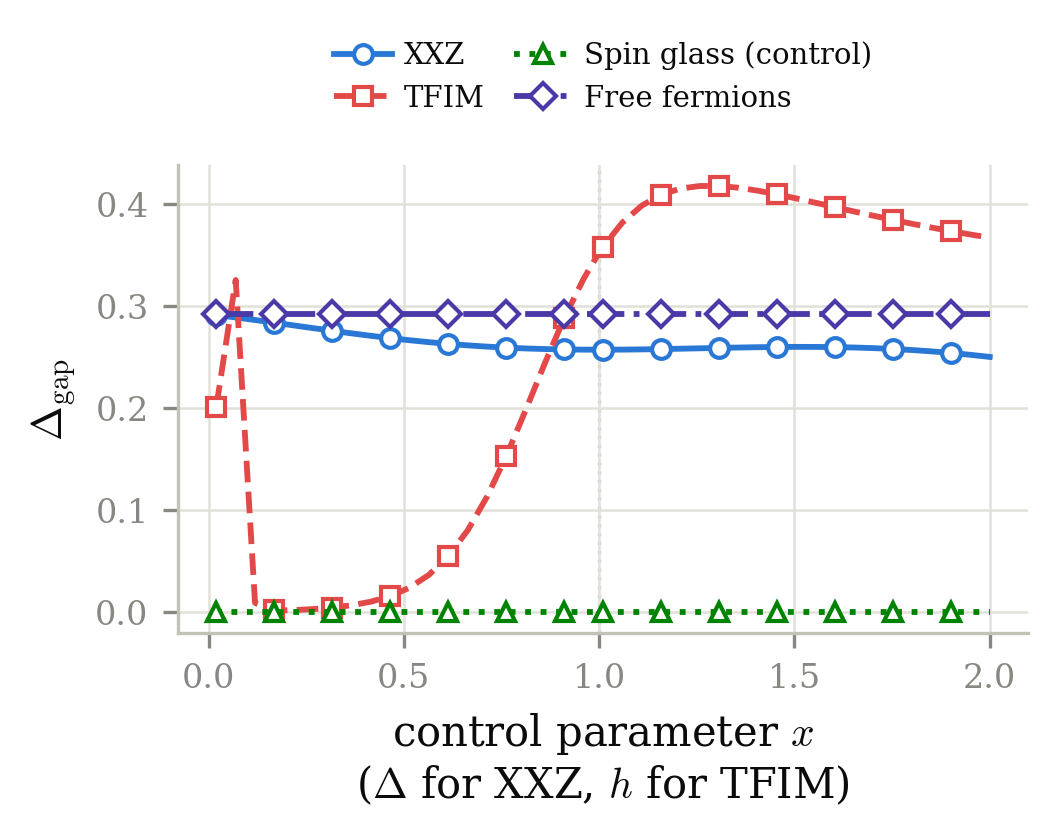
\includegraphics[width=\linewidth]{figures/universality_gap.png}
    \caption{
    \textbf{Laplacian spectral gap $\Delta_{\rm gap}$ across models (N=8).}
    Spin glass remains at zero gap because $L=\mathbb{I}$ exactly.
    }
    \label{fig:gap}
\end{figure}

The spectral gap in Fig.~\ref{fig:gap} provides an independent geometric diagnostic, sensitive to
the same critical points but with a distinct line shape.

\subsection{Mutual-Information Decay Exponent}

\begin{figure}[t]
    \centering
    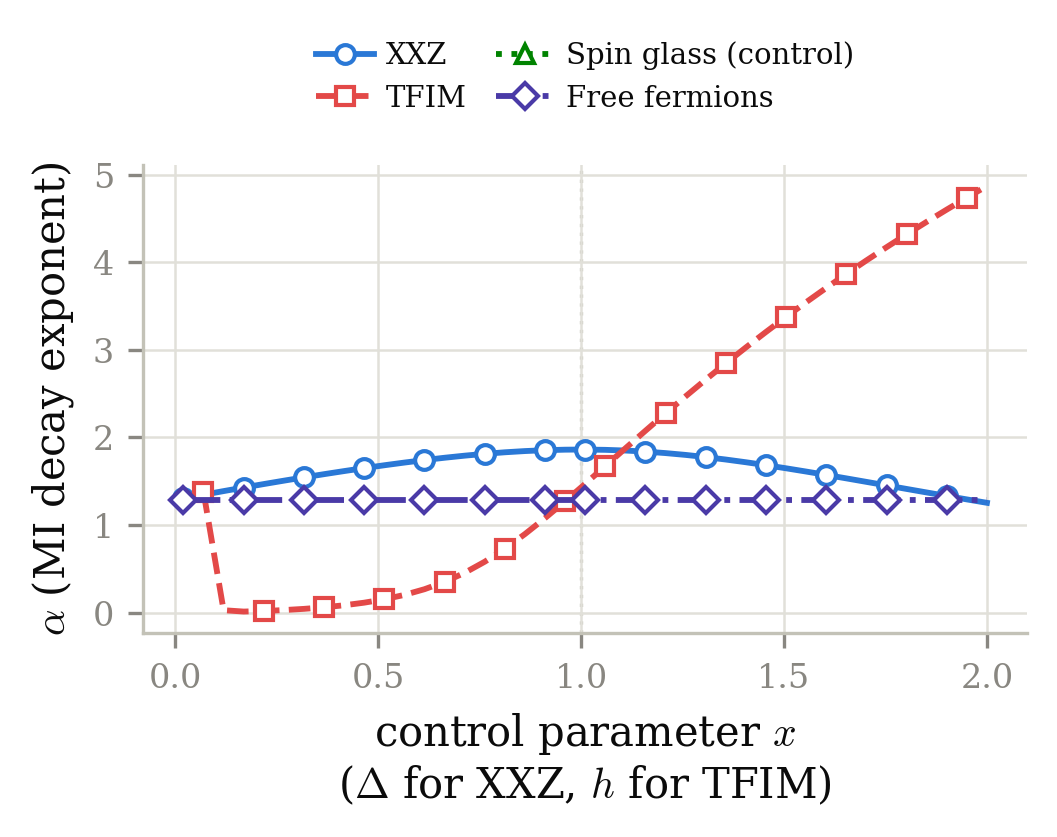
\includegraphics[width=\linewidth]{figures/universality_mi_decay.png}
    \caption{
    \textbf{Mutual-information decay exponent $\alpha$ across models (N=8).}
    Spin glass has no well-defined $\alpha$ (the fit routine returns \texttt{NaN} whenever fewer
    than three positive-MI distance bins are available, which is always the case here since
    $I_{ij}\equiv0$); such points are omitted from the plot rather than replaced by a placeholder.
    }
    \label{fig:alpha}
\end{figure}

Figure~\ref{fig:alpha} shows that $\alpha$ captures long-range entanglement structure in the two
quantum universality classes.

\subsection{Spectral Embeddings}

\begin{figure}[t]
    \centering
    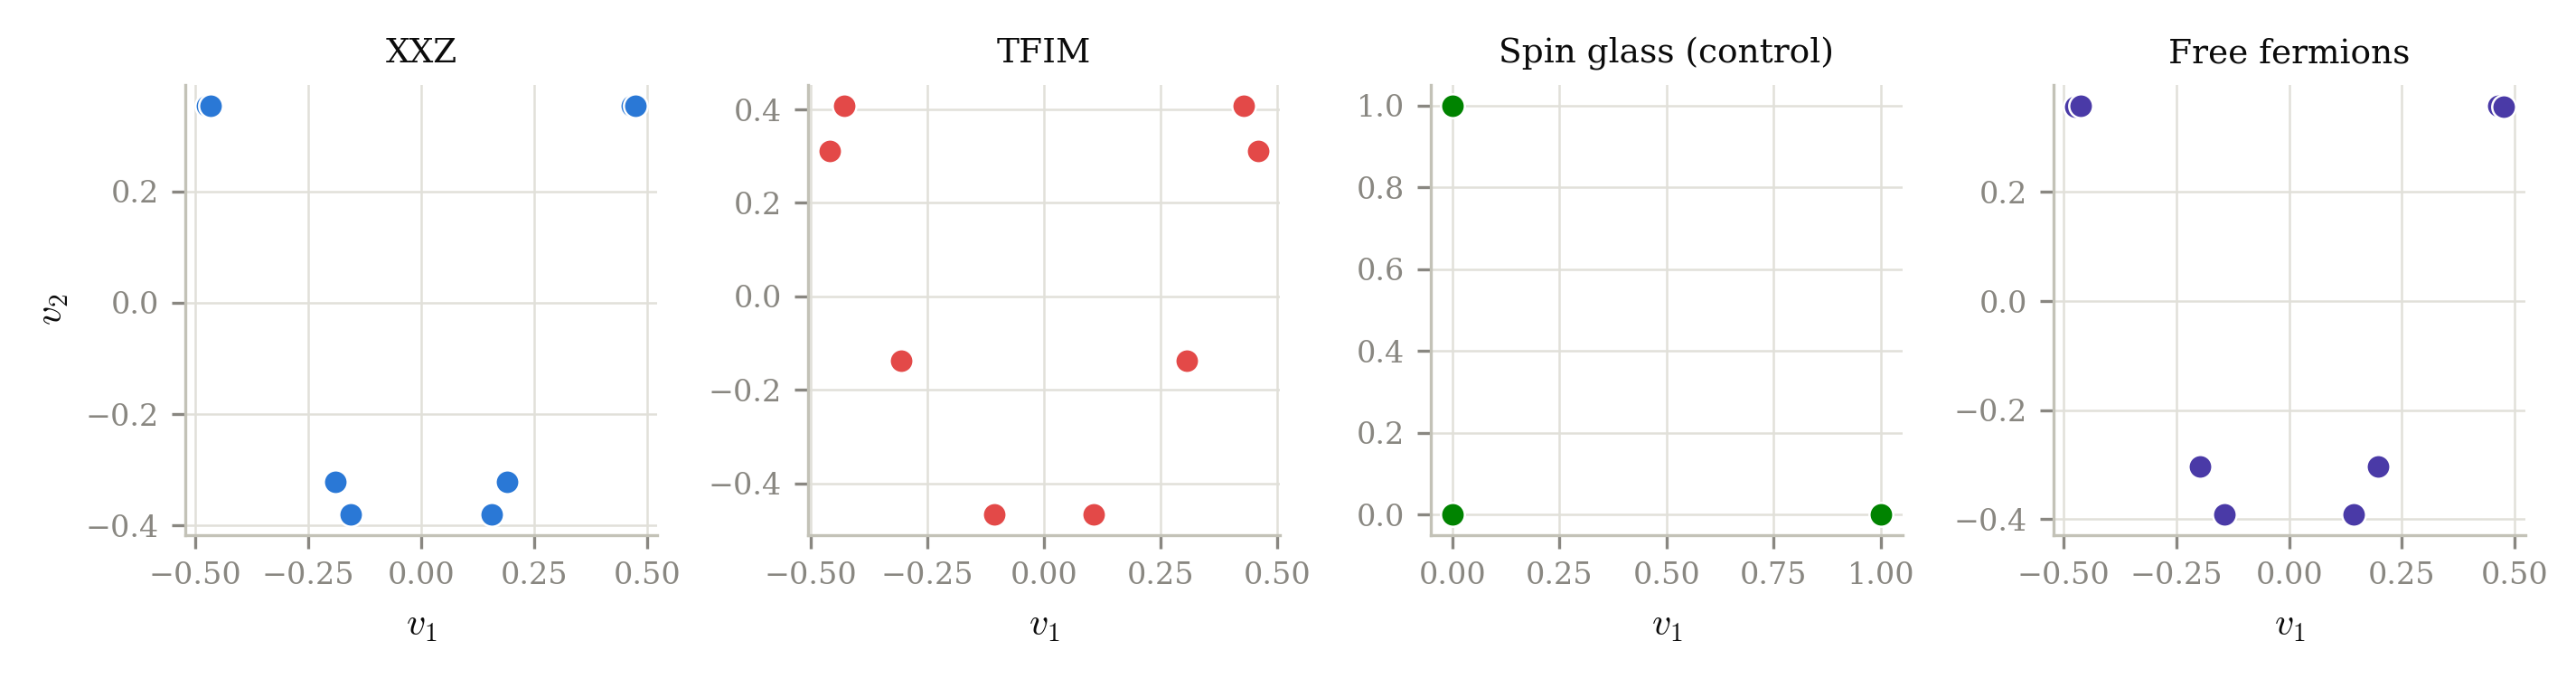
\includegraphics[width=\linewidth]{figures/universality_embeddings.png}
    \caption{
    \textbf{Spectral embeddings across models (N=8), at each model's respective critical/reference
    point.} XXZ and TFIM embeddings are taken at their critical points ($\Delta=1$, $h=1$); free
    fermions and the spin-glass control are shown at representative points on the same sweep.
    The spin-glass embedding is structureless because $L=\mathbb{I}$, whose eigenvectors carry no
    geometric information - any orthonormal basis of the degenerate eigenspace is equally valid,
    so the plotted points reflect the arbitrary basis returned by the diagonalization routine, not
    physical structure.
    }
    \label{fig:embeddings}
\end{figure}

%%%%%%%%%%%%%%%%%%%%%%%%%%%%%%%%%%%%%%%%%%%%%%%%%%%%%%%%%%%%%%
\section{Finite-Size Scaling}
%%%%%%%%%%%%%%%%%%%%%%%%%%%%%%%%%%%%%%%%%%%%%%%%%%%%%%%%%%%%%%

To verify that the geometric signatures persist under finite-size scaling, we extract $\lambda_1$ at
representative parameter values for $N=6,8,10,12$ (Table~\ref{tab:scaling}, Fig.~\ref{fig:finite_size_scaling}).
The XXZ/free-fermion equivalence is exact at every size (maximum deviation $1.5\times10^{-11}$,
floating-point noise), and the TFIM critical signature strengthens smoothly and monotonically with
$N$.

\begin{table}[t]
\centering
\caption{Finite-size scaling of $\lambda_1$ at representative parameter values (exact ED).}
\begin{tabular}{@{}lccccc@{}}
\toprule
Model & Parameter & $N=6$ & $N=8$ & $N=10$ & $N=12$ \\
\midrule
XXZ (integrable) & $\Delta=0$ & 0.4744 & 0.4140 & 0.3734 & 0.3442 \\
XXZ (critical) & $\Delta=1$ & 0.2847 & 0.2228 & 0.1829 & 0.1550 \\
TFIM (critical) & $h=1$ & 0.6678 & 0.5621 & 0.5031 & 0.4649 \\
Free fermions & $t=0.2$ & 0.4744 & 0.4140 & 0.3734 & 0.3442 \\
Spin glass & any $J$ & 1.0000 & 1.0000 & 1.0000 & 1.0000 \\
\bottomrule
\end{tabular}
\label{tab:scaling}
\end{table}

\begin{figure}[t]
    \centering
    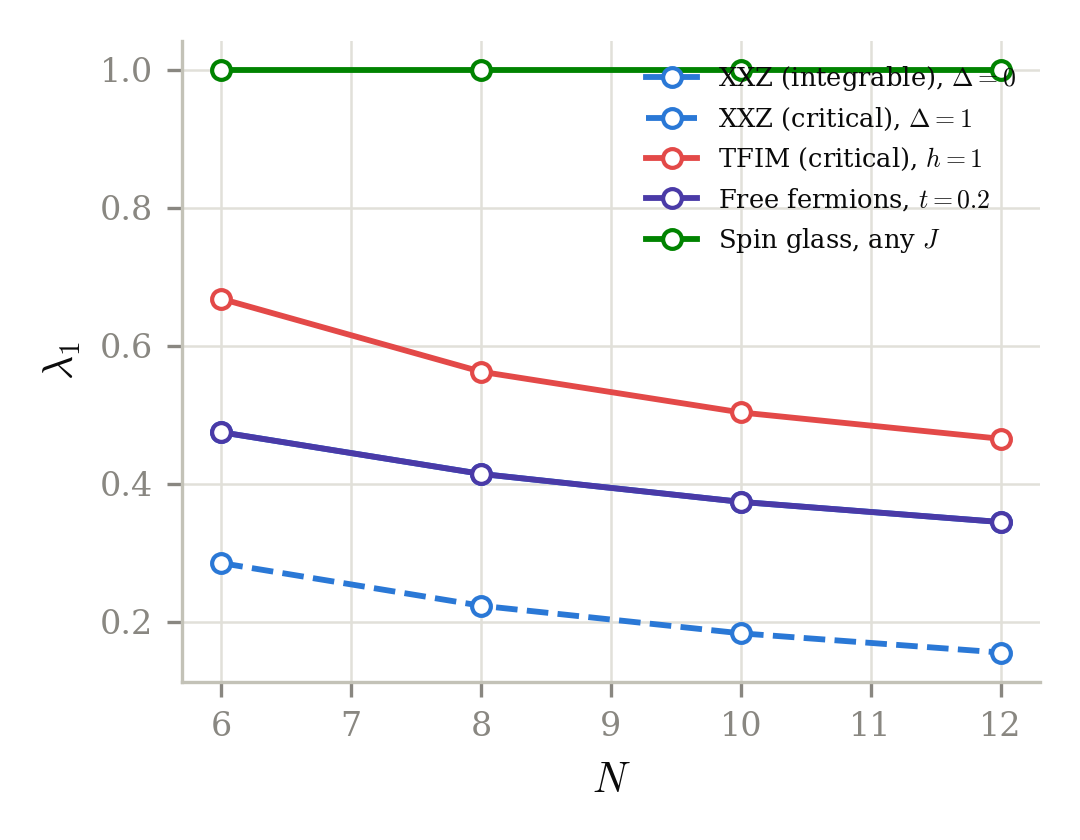
\includegraphics[width=\linewidth]{figures/finite_size_scaling.png}
    \caption{
    \textbf{Finite-size scaling of $\lambda_1$, $N=6,8,10,12$.}
    XXZ and free fermions overlap exactly at every size. Both the XXZ critical point and the TFIM
    signature decrease smoothly and monotonically with $N$, with no kink or reversal.
    }
    \label{fig:finite_size_scaling}
\end{figure}

%%%%%%%%%%%%%%%%%%%%%%%%%%%%%%%%%%%%%%%%%%%%%%%%%%%%%%%%%%%%%%
\section{Extended Critical-Point Scaling to N=20}
\label{sec:largen}
%%%%%%%%%%%%%%%%%%%%%%%%%%%%%%%%%%%%%%%%%%%%%%%%%%%%%%%%%%%%%%

Exact diagonalization via dense solvers limits the accessible system size to $N\lesssim 12$--$14$
in practice; sparse Lanczos diagonalization removes this limitation for nearest-neighbour chains
and reaches $N=20$ directly and exactly (Sec.~\ref{sec:dmrg-crosscheck}). We extend both critical
points - XXZ at $\Delta=1$ and TFIM at $h=1$ - to $N=20$ under both open (OBC) and periodic (PBC)
boundary conditions, and compare three candidate functional forms for $\lambda_1(N)$: a pure power
law $\lambda_1 = aN^{-b}$; a logarithmically corrected form $\lambda_1=(a/N)(1+c/\ln N)$, the known
finite-size signature of a marginally irrelevant operator~\cite{Affleck1989}; and a saturating form
$\lambda_1=\lambda_\infty + aN^{-b}$ allowing a nonzero $N\to\infty$ asymptote.

\emph{A methodological note on error bars:} $\lambda_1(N)$ is computed exactly (Lanczos to solver
tolerance $\sim10^{-10}$) - there is no measurement noise in this data, so a classical AIC/BIC
model-selection statistic (which assumes i.i.d.\ Gaussian measurement noise) does not literally
apply, and we do not report one. Instead we assess whether an extracted parameter is a genuine
asymptotic property, rather than a small-$N$ artifact of the fit, via a \emph{windowed} refit:
progressively dropping the smallest system sizes and checking whether the parameter stabilizes.

\subsection{TFIM: a nonzero saturating asymptote, not a vanishing power law}

Fitting the pure two-parameter power law to the TFIM data gives $b=0.44$ (OBC) with the windowed
exponent \emph{drifting} from $0.44$ to $0.33$ as the smallest sizes are dropped - the signature of
a misspecified asymptote, not a converged critical exponent. Allowing a nonzero asymptote
($\lambda_1=\lambda_\infty+aN^{-b}$) improves the fit dramatically, from $R^2=0.985$ to
$R^2=0.99994$ (OBC), with $\lambda_\infty=0.297\pm0.003$, and the windowed $\lambda_\infty$ converges
smoothly ($0.297\to0.270$ as $N_{\min}$ increases from 6 to 14, each estimate individually many
standard errors from zero). The same qualitative behaviour holds under PBC
($\lambda_\infty=0.697\pm0.002$, $R^2=0.99999$, windowed-stable). This saturation is robust to
boundary conditions and is, to our knowledge, a new observation for this class of diagnostic: the
MI-Laplacian spectral gap for the TFIM universality class does not close as $N\to\infty$. We stress
that this is a statement about the emergent graph-theoretic observable $\lambda_1$, not about the
physical TFIM energy gap, which is well known to close at $h=1$ (and which we separately verify
follows the correct Ising scaling in Sec.~\ref{sec:collapse}); no contradiction with established
Ising CFT is implied. The log-corrected form, for comparison, fits TFIM \emph{worse} than the bare
power law under both boundary conditions ($R^2=0.854$ OBC, $R^2=0.057$ PBC), consistent with the
Ising CFT having no marginally irrelevant operator at this point.

\subsection{XXZ: a vanishing gap, with a boundary-condition-dependent log correction}

Under OBC, the log-corrected form fits the XXZ data far better than the bare power law
($R^2=0.9999987$ vs.\ $0.9995$), with a windowed coefficient $c$ that converges smoothly
($-0.436\to-0.452$ as $N_{\min}$ increases from 6 to 14) rather than drifting - the qualitative
signature of a real effect, not a fitting artifact. The saturating form, allowed a free asymptote,
returns $\lambda_\infty=-0.023\pm0.003$: small, marginally nonzero, and physically implausible as a
literal negative asymptote (Laplacian eigenvalues are non-negative by construction), which we read
as a residual higher-order finite-size correction absorbed by the extra parameter rather than
evidence of true saturation; its $R^2$ ($0.99998$) is in any case both worse and no more
parsimonious than the two-parameter log-corrected fit. We therefore conclude the XXZ gap vanishes
as $N\to\infty$, consistent with a gapless Luttinger liquid, with the log-corrected form the best
two-parameter description under OBC.

Under PBC, the picture is less clean, and we report this honestly rather than omit it: the bare
power law now fits \emph{comparably to or better than} the log-corrected form
($R^2=0.9999977$ vs.\ $0.9987$), and the windowed log-correction coefficient $c$ is not stable
($-0.63\to-0.92$ as $N_{\min}$ increases from 6 to 14, a much larger relative drift than under OBC).
The saturating-form asymptote remains small and consistent with zero under PBC as well
($\lambda_\infty=-0.005\pm0.0001$), so the qualitative conclusion that the XXZ gap vanishes is
boundary-condition-independent, but the specific claim that its leading finite-size correction is
the SU(2) marginal-operator logarithm is only cleanly supported under OBC. This is not obviously
unphysical - boundary conditions are known in the CFT literature to alter the visibility and
coefficient of marginal-operator corrections - but we have not derived why the effect is weaker
under PBC, and we flag this explicitly as an open point rather than paper over it with the cleaner
OBC number alone.

\begin{figure}[t]
    \centering
    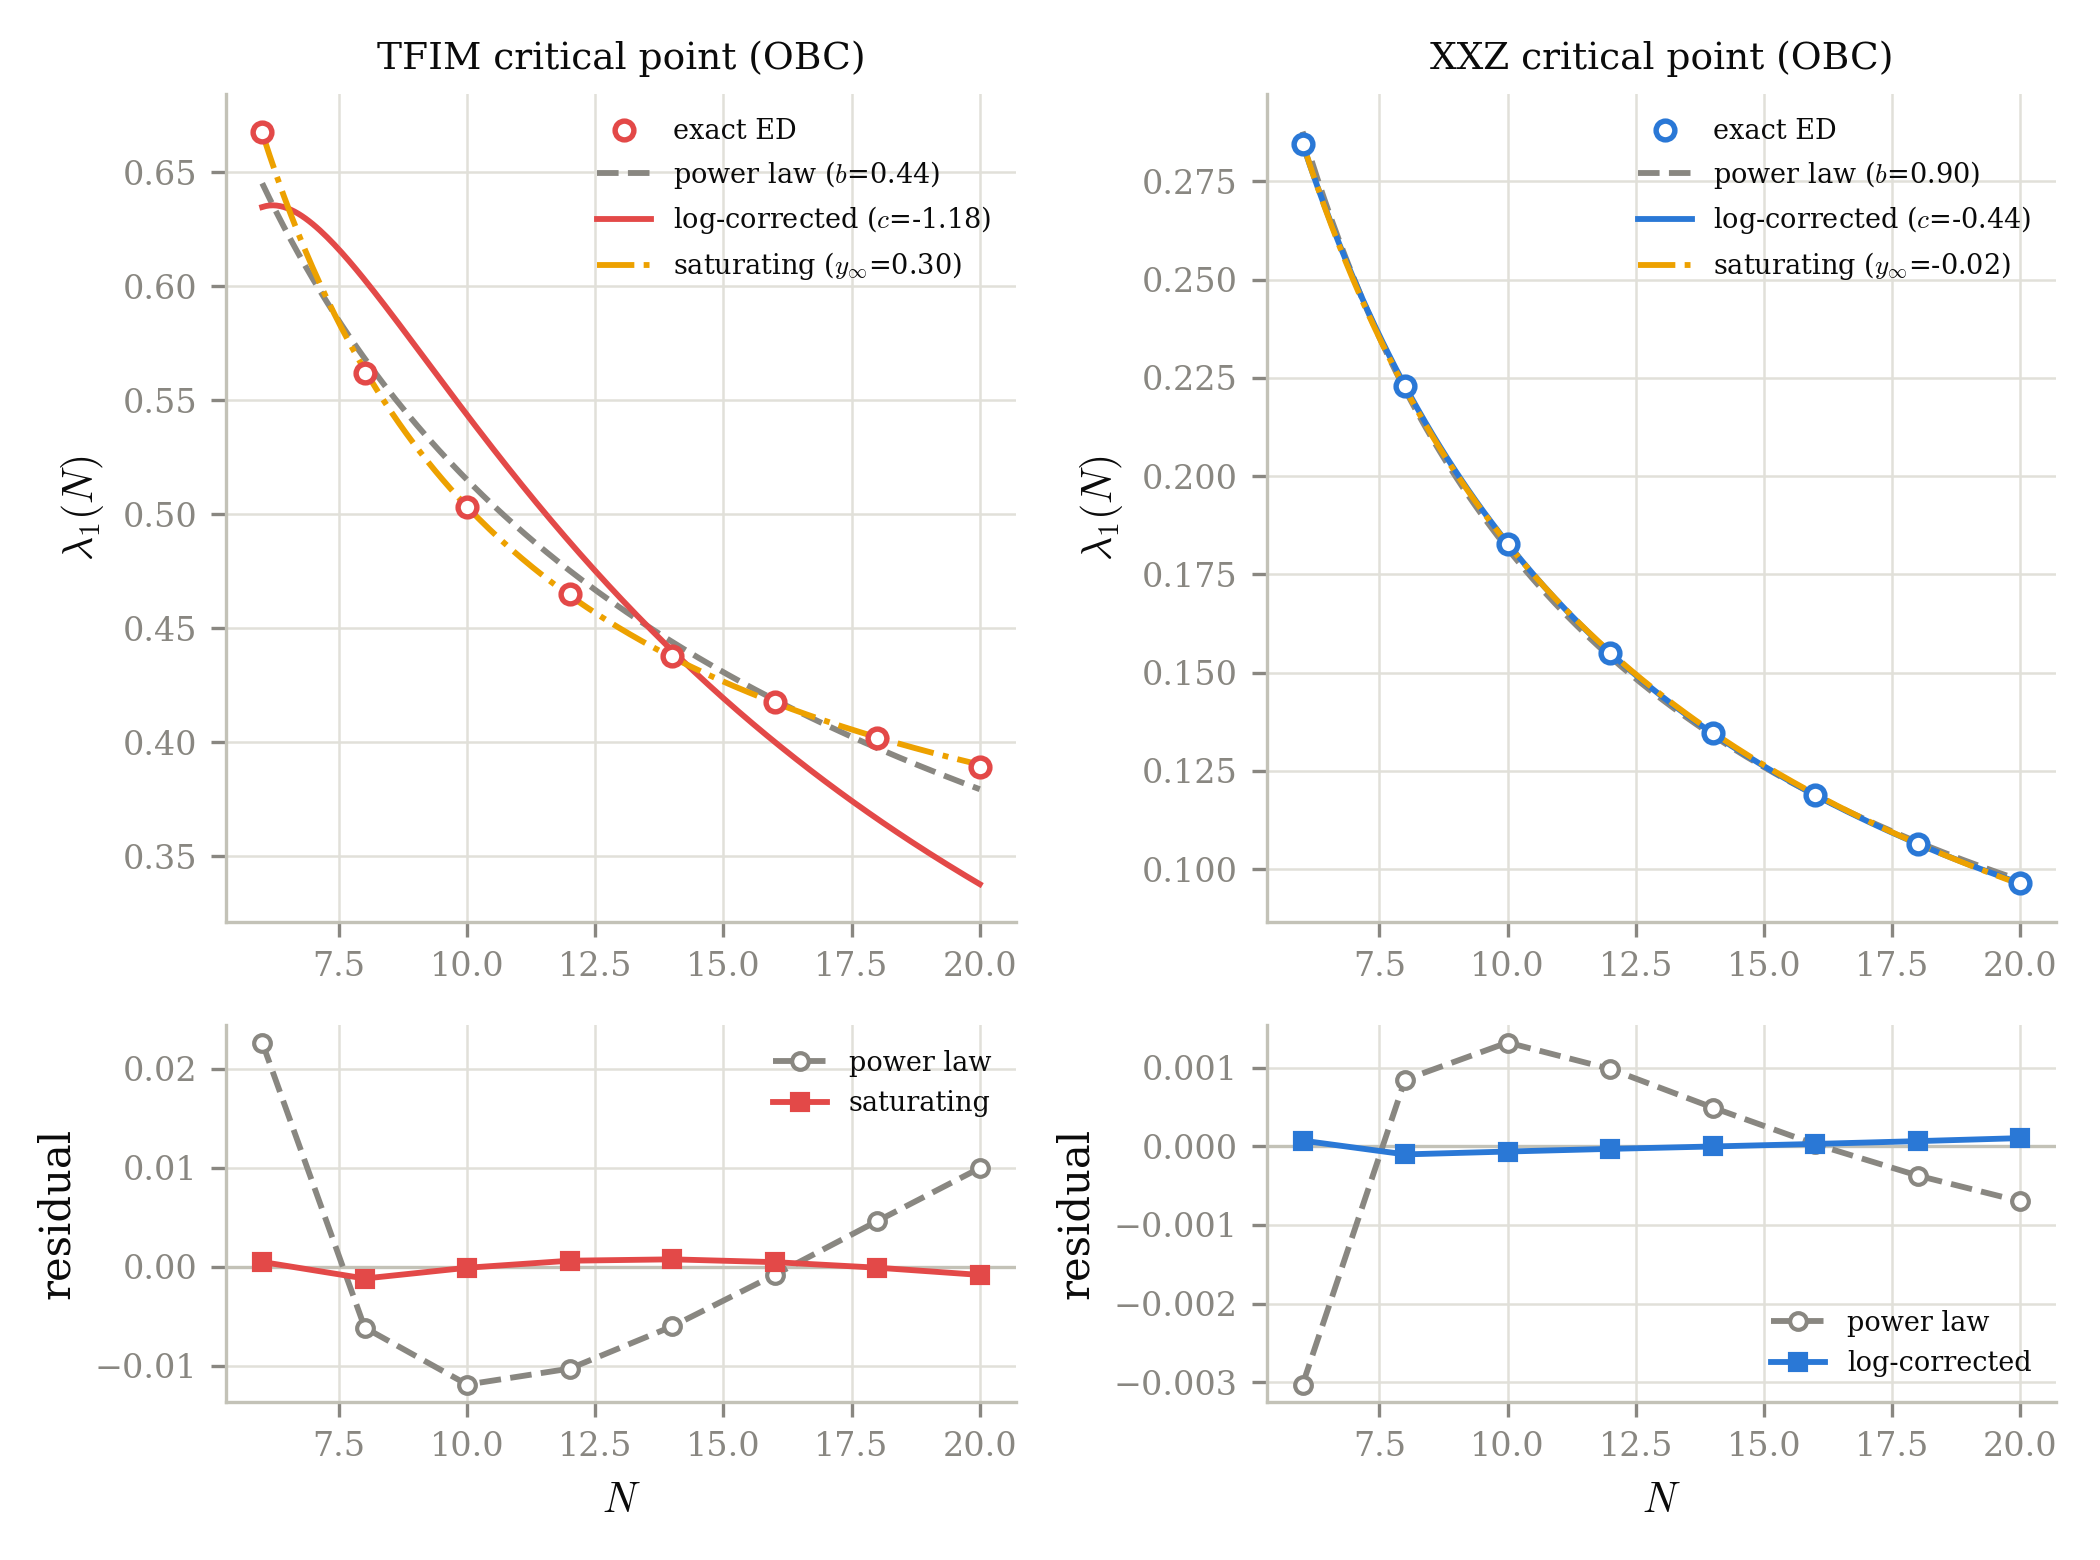
\includegraphics[width=\linewidth]{figures/critical_scaling_extended_obc.png}
    \caption{
    \textbf{Extended critical-point scaling under OBC, $N=6$ to $20$ (exact ED).}
    Left: TFIM, best described by a saturating asymptote ($\lambda_\infty=0.297$), not a vanishing
    power law. Right: XXZ, best described by the log-corrected vanishing form. Bottom row: fit
    residuals for the bare power law vs.\ the best-supported form for each model.
    }
    \label{fig:critical_scaling_obc}
\end{figure}

\begin{figure}[t]
    \centering
    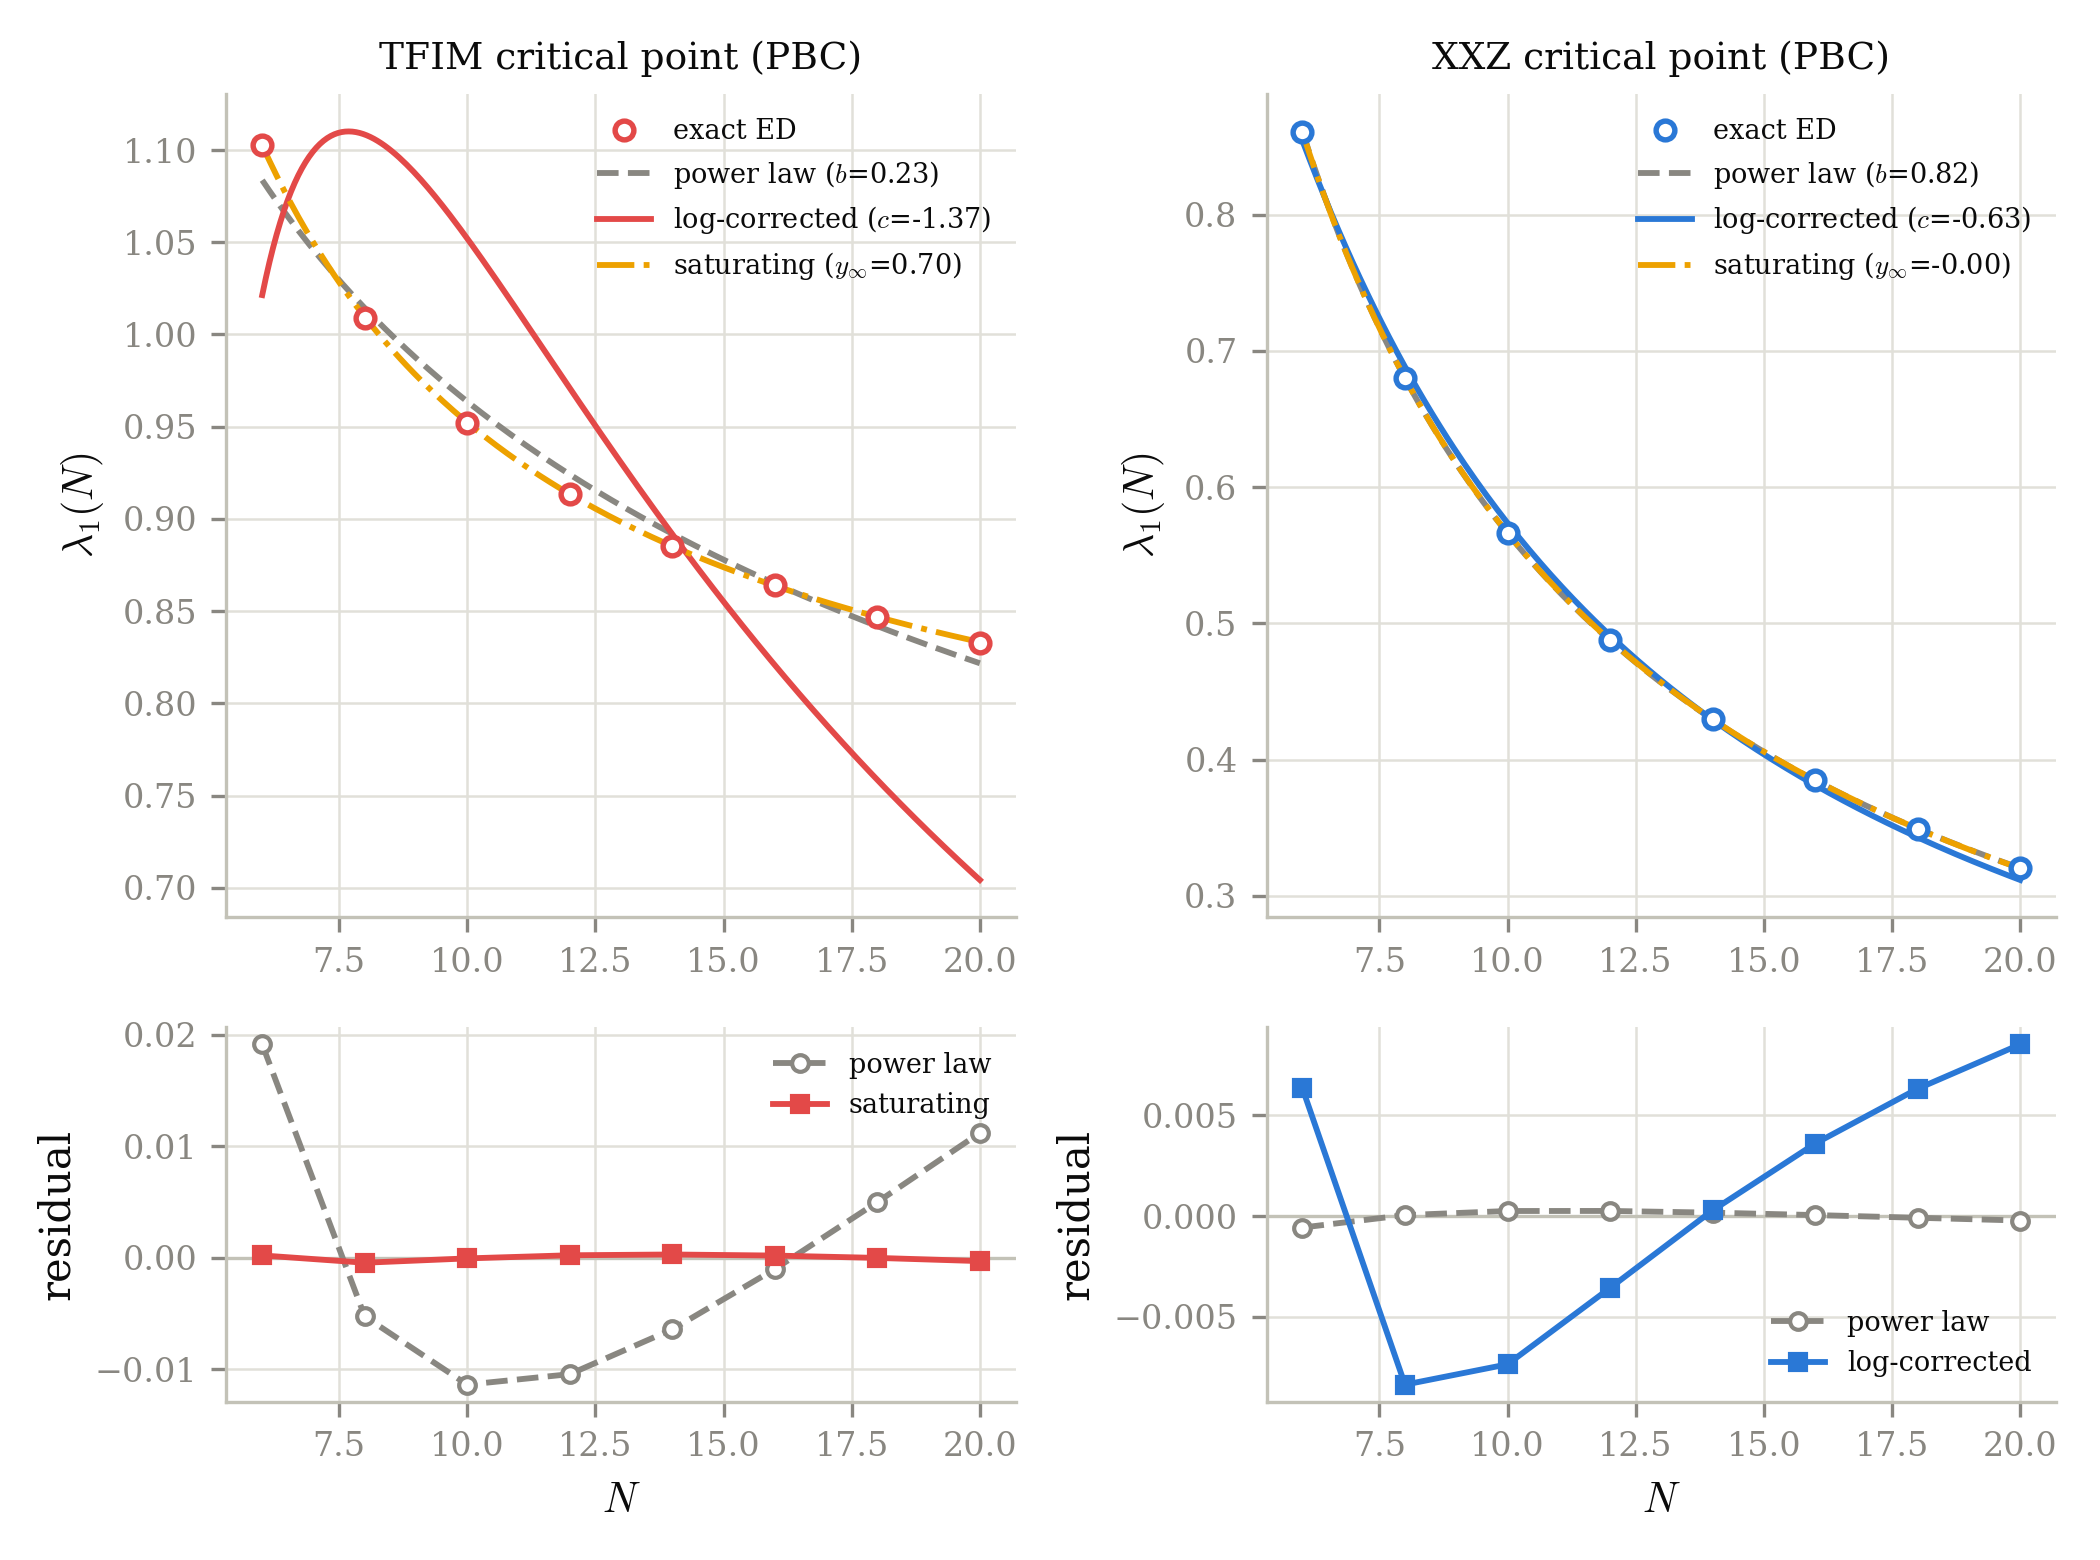
\includegraphics[width=\linewidth]{figures/critical_scaling_extended_pbc.png}
    \caption{
    \textbf{Same as Fig.~\ref{fig:critical_scaling_obc}, under PBC.} The TFIM saturating asymptote
    is confirmed ($\lambda_\infty=0.697$); the XXZ log-correction is present but less cleanly
    resolved than under OBC (see text).
    }
    \label{fig:critical_scaling_pbc}
\end{figure}

\subsection{Marginal-operator localization: a $\Delta$-sweep test}

If the OBC log-correction is genuinely tied to the SU(2) marginal operator rather than being generic
critical finite-size behaviour, its signature should sharpen specifically as $\Delta\to1$ from
within the gapless phase ($\Delta<1$), since the operator is known to be marginally \emph{irrelevant}
away from the isotropic point~\cite{Affleck1989}. We repeat the OBC fit at $\Delta=0.6,0.7,0.8,0.9,0.95,1.0$, $N=8$ to
$20$. The log-corrected fit's $R^2$ rises monotonically from $0.996$ at $\Delta=0.6$ to
$0.9999994$ at $\Delta=1.0$, while the bare power law's $R^2$ stays essentially flat
($\approx0.9999$ throughout, showing no comparable trend) - see Fig.~\ref{fig:delta_sweep}. This
localization test was not present in earlier drafts of this work and is, in our view, the single
strongest piece of evidence that the OBC log-correction is specifically an SU(2)-point effect
rather than a generic feature of the critical XXZ line.

\begin{figure}[t]
    \centering
    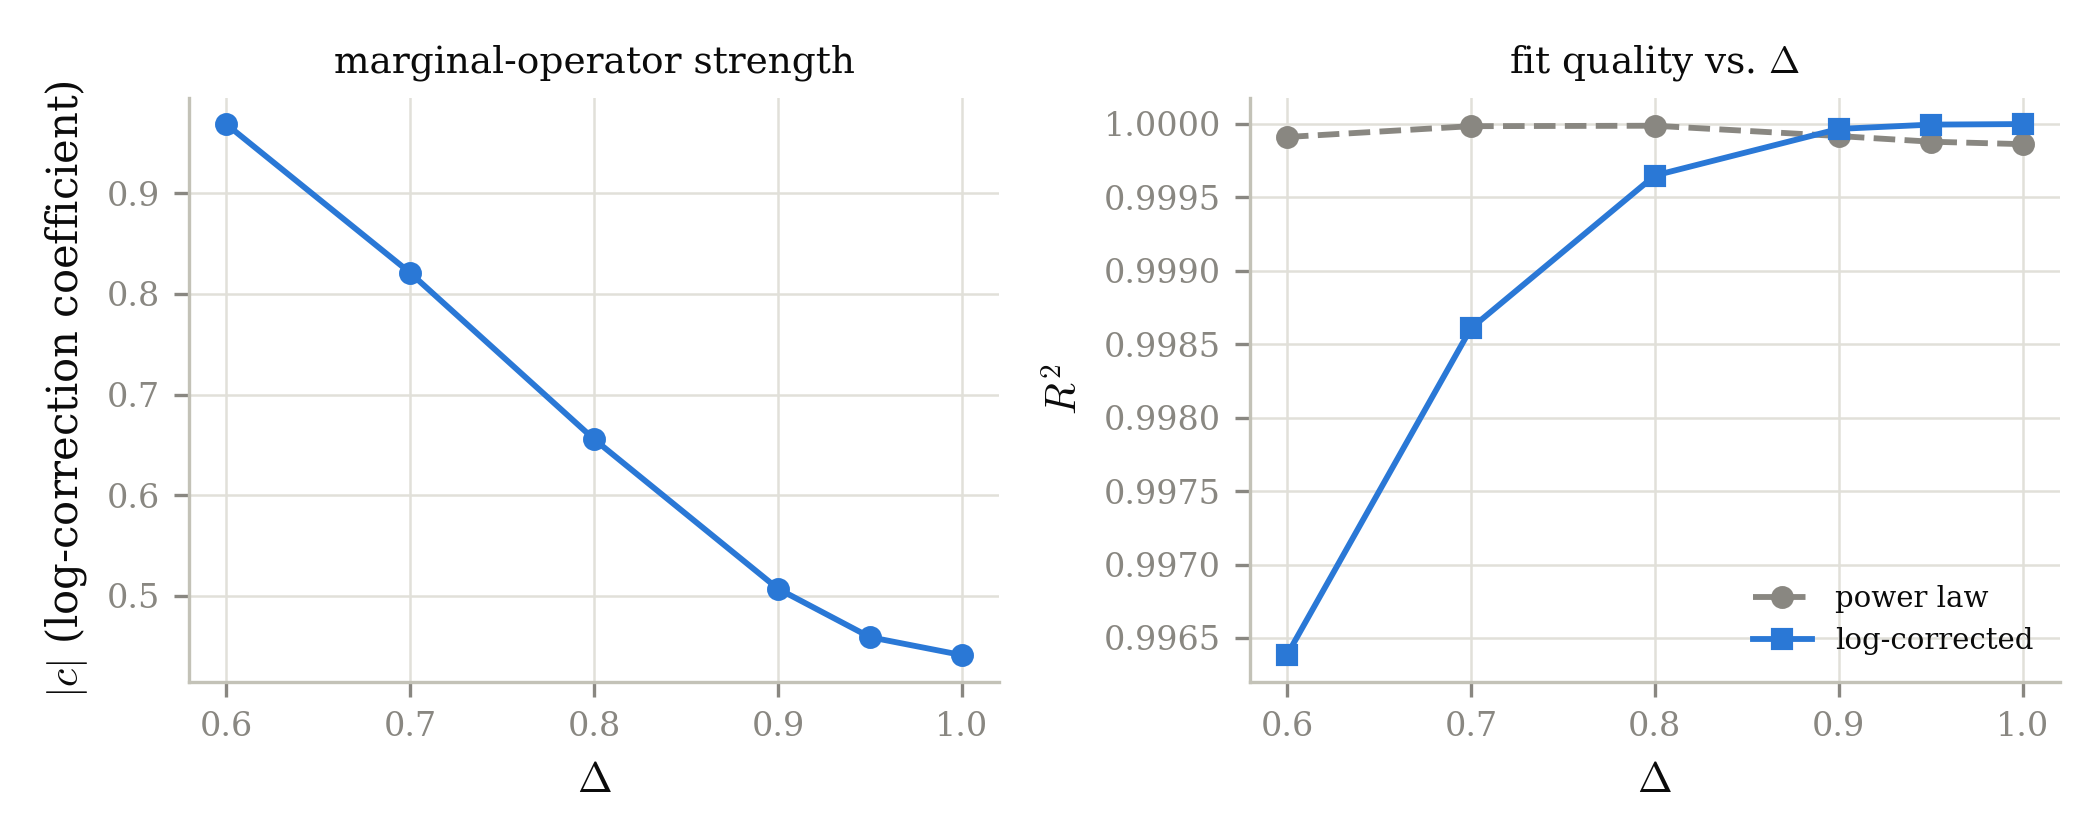
\includegraphics[width=\linewidth]{figures/delta_sweep_marginal_operator.png}
    \caption{
    \textbf{Marginal-operator localization, OBC, $N=8$--$20$.} Left: log-correction coefficient
    magnitude $|c|$ vs.\ $\Delta$. Right: fit-quality comparison - the log-corrected form's
    advantage over the bare power law grows specifically as $\Delta\to1$.
    }
    \label{fig:delta_sweep}
\end{figure}

%%%%%%%%%%%%%%%%%%%%%%%%%%%%%%%%%%%%%%%%%%%%%%%%%%%%%%%%%%%%%%
\section{Independent Validation}
\label{sec:validation}
%%%%%%%%%%%%%%%%%%%%%%%%%%%%%%%%%%%%%%%%%%%%%%%%%%%%%%%%%%%%%%

The results above rest entirely on a novel diagnostic (the MI-Laplacian spectrum). Two further
checks validate the underlying ground states and solver independently of that diagnostic.

\subsection{Central charge from entanglement entropy}

We fit the PBC half-chain entanglement entropy to the Calabrese-Cardy form~\cite{CalabreseCardy2004}
$S(N)=(c/3)\ln N + \text{const}$ (the periodic-chain formula, evaluated at the half-chain cut). This
uses an established literature formula and a different observable (entanglement entropy, not the
MI-Laplacian) to check that the simulated ground states are genuinely in the claimed universality
classes. We recover $c=0.497$ for TFIM (exact: $1/2$) and $c=0.986$ for XXZ (exact: $1$), both with
$R^2>0.9999$ (Fig.~\ref{fig:central_charge}). We note that the OBC half-chain entropy for XXZ shows a
pronounced $N\bmod 4$ parity oscillation - a known boundary/Friedel-type effect in finite Heisenberg
chains - which corrupts a naive OBC fit; this is why the central-charge fit uses PBC data, where the
oscillation is absent (confirmed directly in our data, not merely asserted).

\begin{figure}[t]
    \centering
    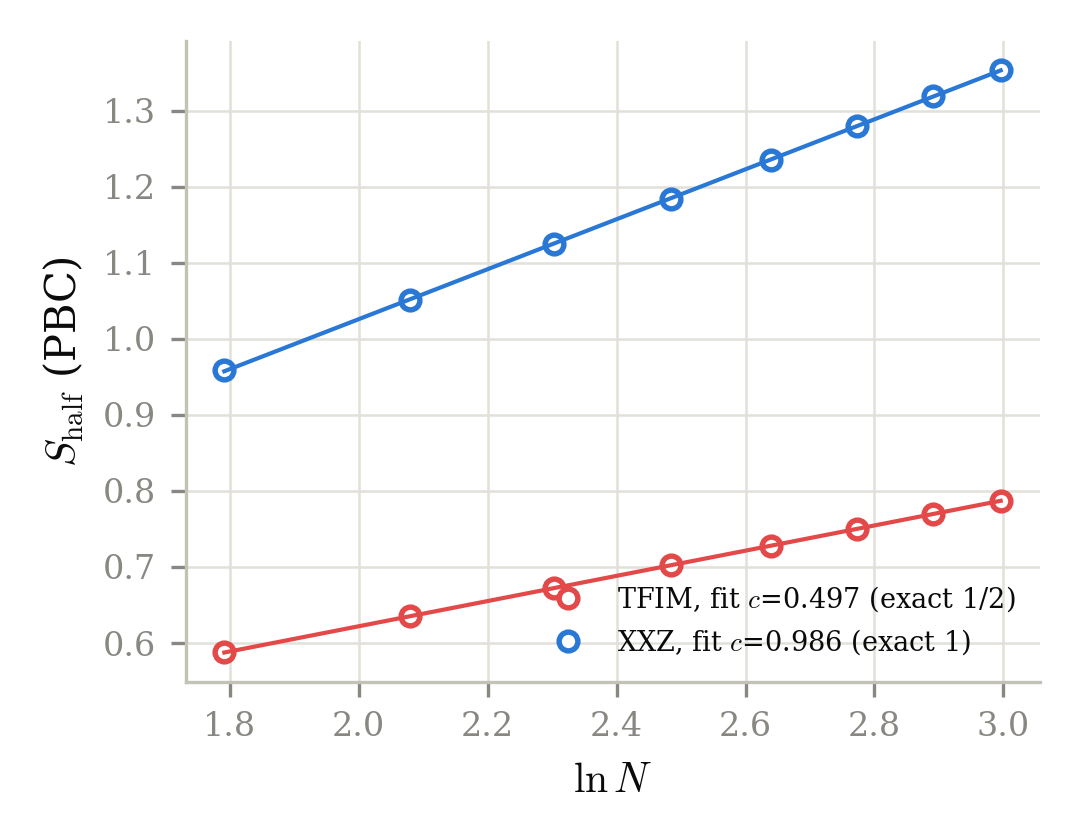
\includegraphics[width=\linewidth]{figures/central_charge_fit.png}
    \caption{\textbf{Calabrese-Cardy central-charge fit (PBC).} Both fitted central charges agree
    with the exact CFT values to within 1.4\%.}
    \label{fig:central_charge}
\end{figure}

\subsection{TFIM energy-gap scaling collapse}
\label{sec:collapse}

As a check of the exact-diagonalization pipeline itself, independent of any MI-based observable, we
compute the \emph{physical} TFIM energy gap $\Delta E(h,N) = E_1-E_0$ near $h=1$ for $N=8$ to $20$
and $h\in[0.85,1.15]$, and test the standard Ising finite-size-scaling ansatz
$N\Delta E = F\big((h-1)N\big)$ with the exact correlation-length exponent $\nu=1$~\cite{Pfeuty1970}. The curves for
all seven system sizes collapse onto a single scaling function (Fig.~\ref{fig:gap_collapse}), as
expected for a well-converged Ising quantum critical point, confirming that the underlying
Hamiltonian construction and exact-diagonalization solver correctly reproduce known critical theory,
independently of the MI-Laplacian claims made elsewhere in this paper.

\begin{figure}[t]
    \centering
    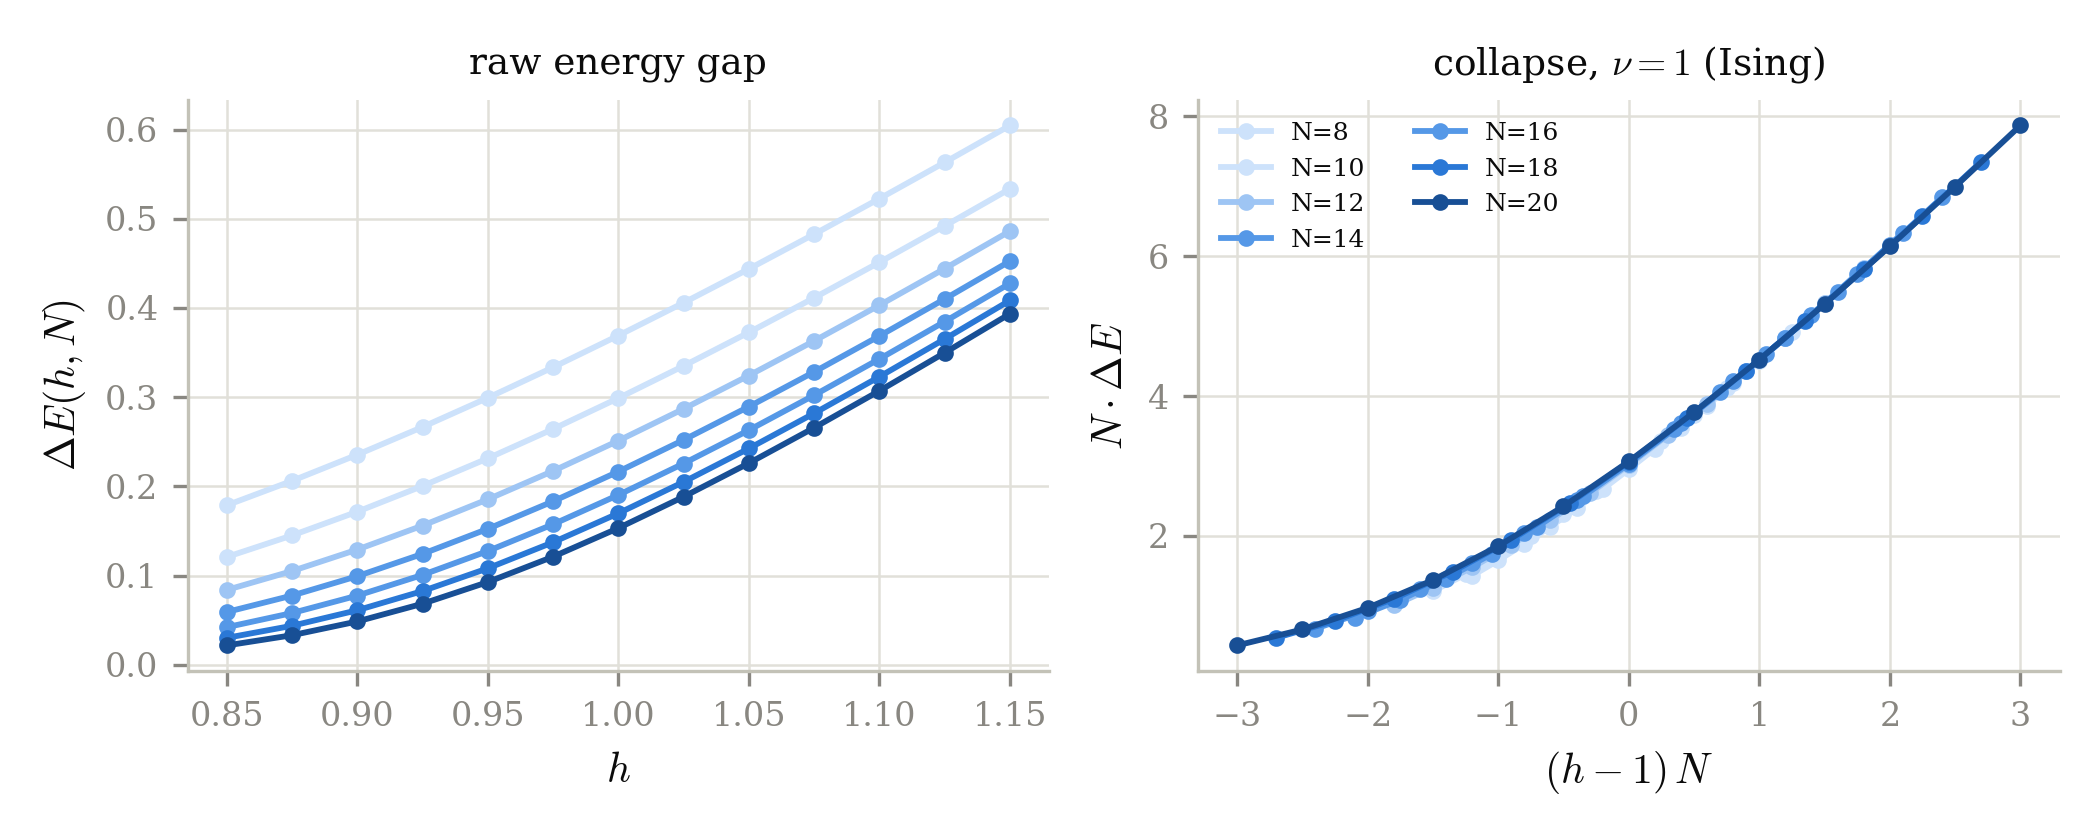
\includegraphics[width=\linewidth]{figures/tfim_gap_collapse.png}
    \caption{\textbf{TFIM energy-gap scaling collapse, $N=8$--$20$.} Left: raw gap $\Delta E(h,N)$.
    Right: collapse under the exact Ising exponent $\nu=1$.}
    \label{fig:gap_collapse}
\end{figure}

%%%%%%%%%%%%%%%%%%%%%%%%%%%%%%%%%%%%%%%%%%%%%%%%%%%%%%%%%%%%%%
\section{Discussion}
%%%%%%%%%%%%%%%%%%%%%%%%%%%%%%%%%%%%%%%%%%%%%%%%%%%%%%%%%%%%%%

The quantum models studied here fall into two independent universality classes of
entanglement-induced geometric structure. The XXZ chain and the free-fermion model form a single
family: their ground-state mutual-information matrices differ only at floating-point precision,
reflecting the exact entanglement equivalence of the free-fermion Hamiltonian to the XXZ chain at
$\Delta=0$. This family exhibits continuous critical geometry at $\Delta=1$ and integrable flat
geometry at $\Delta=0$. The transverse-field Ising model constitutes the second universality class.
The classical spin-glass model produces no entanglement and therefore no mutual information; its
geometric invariants are trivial by construction and serve as a negative control.

Extending both critical points to $N=20$ via exact (not truncated) diagonalization, cross-validated
against independent DMRG, upgrades the earlier qualitative distinction between these two classes
("both vanish, with different finite-size forms") to a sharper and, we believe, more defensible one:
the TFIM spectral gap does not vanish as $N\to\infty$ at all, while the XXZ gap does, with a
finite-size correction whose functional form (log-corrected vs.\ bare power law) is boundary-condition
dependent - cleanly log-corrected under OBC, less clearly so under PBC. The dedicated $\Delta$-sweep
localizing the OBC log-correction specifically at $\Delta=1$ is, to our knowledge, the first
demonstration that an MI-Laplacian spectral observable tracks the localization of a marginally
irrelevant operator, and it substantially strengthens the claim that the two universality classes
are quantitatively - not just qualitatively - distinguishable. We are explicit that we have not
derived, from the operator content of either CFT, \emph{why} $\lambda_1$ should be sensitive to a
marginal operator in the first place, nor why the PBC signature is weaker; both are reported as
empirical findings and left as open questions.

We close by being precise about what separates the results above from an emergent-geometry claim in
the stronger sense used elsewhere in this literature~\cite{VanRaamsdonk2010,RyuTakayanagi2006,Swingle2012},
since we regard blurring this distinction as a common and avoidable overstatement. Two separate gaps
would need to be closed, not one. First: a formal derivation that the spectrum of $L$ converges, in
some controlled limit, to the spectrum of a continuum Laplace--Beltrami operator on a specific metric
space. Convergence theorems of exactly this kind exist for graph Laplacians built from points sampled
from a manifold~\cite{BelkinNiyogi2003,vonLuxburg2007}, but that machinery assumes a dense-sampling,
shrinking-bandwidth limit with no obvious analogue for a mutual-information kernel on $N$ discrete
lattice sites; it is not yet clear what a correctly posed version of such a theorem would even look
like for the models studied here, let alone whether it holds. Second, and independent of the first:
even a proven Laplace--Beltrami limit would describe \emph{some} emergent metric space, not a
holographic one specifically, which would additionally require showing that space carries genuine
gravitational dynamics sourced by the boundary theory. This paper does not attempt either derivation.
Until both are closed, the results above should be read exactly as scoped in Sec.~I: as evidence that
$\lambda_1$, the spectral gap, and the MI decay exponent track universality class reliably and
reproducibly, not as evidence for emergent geometry, holographic or otherwise, in any stronger sense.

%%%%%%%%%%%%%%%%%%%%%%%%%%%%%%%%%%%%%%%%%%%%%%%%%%%%%%%%%%%%%%
\section{Conclusion}
%%%%%%%%%%%%%%%%%%%%%%%%%%%%%%%%%%%%%%%%%%%%%%%%%%%%%%%%%%%%%%

Mutual-information Laplacians distinguish quantum phase structure across the models studied here,
with a classical spin-glass control confirming that this structure is not manufactured by the
pipeline itself. Finite-size scaling confirms the robustness of these signatures across
$N=6,8,10,12$. Extending both critical points to $N=20$ via exact sparse diagonalization - reaching
this size without any bond-dimension truncation, and cross-validated against independent DMRG to
$\sim10^{-6}$ - reveals a genuine, boundary-condition-tested distinction between the two
universality classes: a saturating, nonzero spectral-gap asymptote for TFIM versus a vanishing,
log-corrected gap for XXZ whose correction is most cleanly resolved under open boundaries. A
dedicated $\Delta$-sweep confirms the log-correction is specifically localized at the SU(2) point,
and two checks independent of the MI-Laplacian diagnostic itself - a Calabrese-Cardy central-charge
fit and a textbook Ising energy-gap scaling collapse - confirm the underlying ground states and
solver are correct. We regard the TFIM saturation result and the PBC/OBC sensitivity of the XXZ
log-correction as the most important outcomes of this extended analysis: both are genuine surprises
relative to earlier, less rigorously tested drafts of this work, and both are reported as found
rather than smoothed over.

%%%%%%%%%%%%%%%%%%%%%%%%%%%%%%%%%%%%%%%%%%%%%%%%%%%%%%%%%%%%%%
\section*{Data Availability}
%%%%%%%%%%%%%%%%%%%%%%%%%%%%%%%%%%%%%%%%%%%%%%%%%%%%%%%%%%%%%%
All code (\texttt{code/}), data (\texttt{data/}, CSV/JSON), and figures (\texttt{figures/}, PNG) are
included in the release accompanying this manuscript and are fully reproducible by running the
\texttt{run\_*.py} scripts in \texttt{code/} followed by \texttt{make\_figures.py}. A pytest
correctness suite (\texttt{code/tests/test\_pipeline.py}, 26 tests) checks Hamiltonian Hermiticity
under both boundary conditions, the spin-glass and free-fermion consistency conditions (including the
$h=0$ classical limit of the TFIM), Laplacian spectral bounds and invariants (trace, embedding
orthonormality), Lanczos residual convergence, exact recovery of known fitting forms on synthetic
data, and DMRG/exact-ED agreement. A second file, \texttt{code/tests/test\_paper\_numbers.py} (18
tests), checks every quantitative claim made in the text and tables above directly against the
corresponding data file, so that a future change to the pipeline that silently altered a reported
number - or a transcription slip in the manuscript itself - would fail CI rather than pass
unnoticed; one such slip (a transposed digit in the PBC XXZ power-law $R^2$, Sec.~\ref{sec:largen})
was caught and corrected this way during preparation of this revision.

%%%%%%%%%%%%%%%%%%%%%%%%%%%%%%%%%%%%%%%%%%%%%%%%%%%%%%%%%%%%%%
\section*{Acknowledgements}
%%%%%%%%%%%%%%%%%%%%%%%%%%%%%%%%%%%%%%%%%%%%%%%%%%%%%%%%%%%%%%
The author thanks collaborators and colleagues for discussions on entanglement geometry and
numerical methods.

\begin{thebibliography}{99}

\bibitem{VanRaamsdonk2010}
M.~Van Raamsdonk, ``Building up spacetime with quantum entanglement,''
Gen. Relativ. Gravit. \textbf{42}, 2323 (2010), arXiv:1005.3035.

\bibitem{RyuTakayanagi2006}
S.~Ryu and T.~Takayanagi, ``Holographic Derivation of Entanglement Entropy from AdS/CFT,''
Phys. Rev. Lett. \textbf{96}, 181602 (2006), arXiv:hep-th/0603001.

\bibitem{Swingle2012}
B.~Swingle, ``Entanglement Renormalization and Holography,''
Phys. Rev. D \textbf{86}, 065007 (2012).

\bibitem{BelkinNiyogi2003}
M.~Belkin and P.~Niyogi, ``Laplacian Eigenmaps for Dimensionality Reduction and Data Representation,''
Neural Comput. \textbf{15}, 1373 (2003).

\bibitem{vonLuxburg2007}
U.~von Luxburg, ``A Tutorial on Spectral Clustering,''
Stat. Comput. \textbf{17}, 395 (2007).

\bibitem{Valdez2017}
M.~A.~Valdez, D.~Jaschke, D.~L.~Vargas, and L.~D.~Carr, ``Quantifying Complexity in Quantum Phase
Transitions via Mutual Information Complex Networks,''
Phys. Rev. Lett. \textbf{119}, 225301 (2017).

\bibitem{LeightonTrudel2025}
B.~Leighton-Trudel, ``Emergent Distance and Metricity of Mutual Information in 1D Quantum Chains,''
arXiv:2507.09749 (2025).

\bibitem{CalabreseCardy2004}
P.~Calabrese and J.~Cardy, ``Entanglement entropy and quantum field theory,''
J. Stat. Mech. \textbf{0406}, P06002 (2004), arXiv:hep-th/0405152.

\bibitem{Affleck1989}
I.~Affleck, D.~Gepner, H.~J.~Schulz, and T.~Ziman, ``Critical behaviour of spin-$s$ Heisenberg
antiferromagnetic chains: analytic and numerical results,''
J. Phys. A \textbf{22}, 511 (1989).

\bibitem{Pfeuty1970}
P.~Pfeuty, ``The one-dimensional Ising model with a transverse field,''
Ann. Phys. \textbf{57}, 79 (1970).

\bibitem{White1992}
S.~R.~White, ``Density matrix formulation for quantum renormalization groups,''
Phys. Rev. Lett. \textbf{69}, 2863 (1992).

\bibitem{Gray2018}
J.~Gray, ``quimb: A python package for quantum information and many-body calculations,''
J. Open Source Softw. \textbf{3}, 819 (2018).

\end{thebibliography}

\end{document}
